But this is just theoretical. The equip of the paper designed real-time peer-to-peer collaborations in order to obtain there logs and apply them on the algorithms. For real applications, two experiments and severals groups have been mades:
\begin{itemize}
	\item 3 grups have to do there semester report only using the collaborating editor during one and a half hours:
		\begin{itemize}
			\item 2 grups of 4 students.
			\item 1 grup of 5 students.
		\end{itemize}
	\item 9 grups of 2 students have to translate an episode of \emph{The Big Bang Theory}
\end{itemize}~

Figure \ref{fig:operations} p.\pageref{fig:operations} shows the total number of users/character operations:
\begin{itemize}
	\item A user operation is adding/deleting letters or grups (copy/past).
	\item A character operaton is the transformation of each user operation into a character operation (for example, copy/past "alma" are the character operations: \begin{itemize}
					\item adding 'a' at space 0
					\item adding 'l' at space 1
					\item ...
				\end{itemize}
\end{itemize}~

\begin{figure}[h]
  \center
  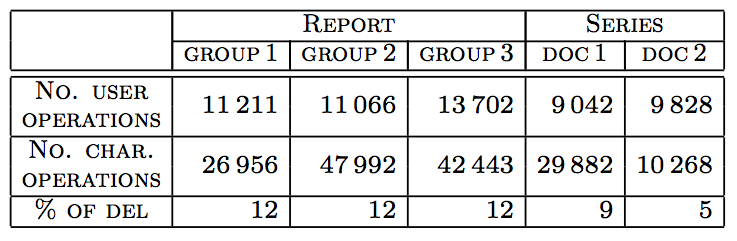
\includegraphics[width=0.7\textwidth]{includes/operations.png}
  \caption{Total number of user/character operations}
  \label{fig:operations}
\end{figure}